\documentclass[a4paper,12pt]{article}
\usepackage[utf8]{inputenc}
\usepackage{geometry}
\usepackage{array}
\usepackage{longtable}
\usepackage{booktabs}
\usepackage{pgfplots} % Para gráficas
\usepackage{float}
\usepackage{hyperref}
\usepackage{fontawesome5}
\pgfplotsset{compat=1.18}
\setlength{\parindent}{0pt}


\geometry{margin=2.5cm}

\title{Experimentos de Estimación de $\pi$ con Programación Paralela y Secuencial}
\author{Juan Diego Collazos Mejia, Juan Sebastian Garizao Puerto, Oscar Vargas Pabon}
\date{August 17, 2025}

\begin{document}

\maketitle

\section*{Descripción}
Este documento recoge los resultados experimentales de tres programas en C++:
\begin{itemize}
    \item \textbf{taylorpi.cpp}: paralelo, método de Taylor (requiere iteraciones y número de hilos).
    \item \textbf{carlopi.cpp}: paralelo, método Monte Carlo (requiere número de lanzamientos y número de hilos).
    \item \textbf{montepi.cpp}: secuencial, método Monte Carlo (requiere número de lanzamientos).
\end{itemize}

Se registraron los tiempos de ejecución:
\begin{itemize}
    \item \textbf{CPU time} medido con \texttt{clock()}.
    \item \textbf{Wall-clock time} medido con \texttt{time()}.
\end{itemize}
Además, se calculó el error absoluto comparando con el valor de \(\pi\) definido en \texttt{math.h}.

\newpage

\section*{Resultados \texttt{taylorpi.cpp} (paralelo -- serie de Taylor)}

\begin{longtable}{>{\raggedright}p{2cm} >{\raggedright}p{1cm} 
>{\centering\arraybackslash}p{3cm} 
>{\centering\arraybackslash}p{3cm} 
>{\centering\arraybackslash}p{2cm} 
>{\centering\arraybackslash}p{3cm}}
\toprule
Iteraciones (N) & Hilos & Tiempo CPU (s) & Tiempo Wall (s) & Valor estimado $\pi$ & Error absoluto \\
\midrule
\endfirsthead
\toprule
Iteraciones (N) & Hilos & Tiempo CPU (s) & Tiempo Wall (s) & Valor estimado $\pi$ & Error absoluto \\
\midrule
\endhead
1e6 & 2 & 0.005381 & 0.0028035 & 3.14159165 & 1.000e-6 \\
1e6 & 4 & 0.005848 & 0.0030669 & 3.14159165 & 1.000e-6 \\
1e6 & 8 & 0.006474 & 0.0019328 & 3.14159165 & 1.000e-6 \\
1e7 & 2 & 0.049728 & 0.0267203 & 3.14159255 & 1.000e-7 \\
1e7 & 4 & 0.046440 & 0.0122906 & 3.14159255 & 1.000e-7 \\
1e7 & 8 & 0.048715 & 0.0069969 & 3.14159255 & 9.999e-8 \\
1e8 & 2 & 0.37089 & 0.187539885 & 3.14159264 & 9.9995425e-9 \\
1e8 & 4 & 0.39799 & 0.108343164 & 3.14159264 & 9.9999759e-9  \\
1e8 & 8 & 0.42705 & 0.077586926 & 3.14159264 & 9.9999133e-9 \\
\bottomrule
\end{longtable}

\begin{center}
    \href{https://github.com/jucollas/parallel-programming/blob/main/submit-I/taylorpi.cpp}{\faGithub\ \texttt{taylorpi.cpp} in GitHub}
\end{center}

\begin{figure}[H]
\centering
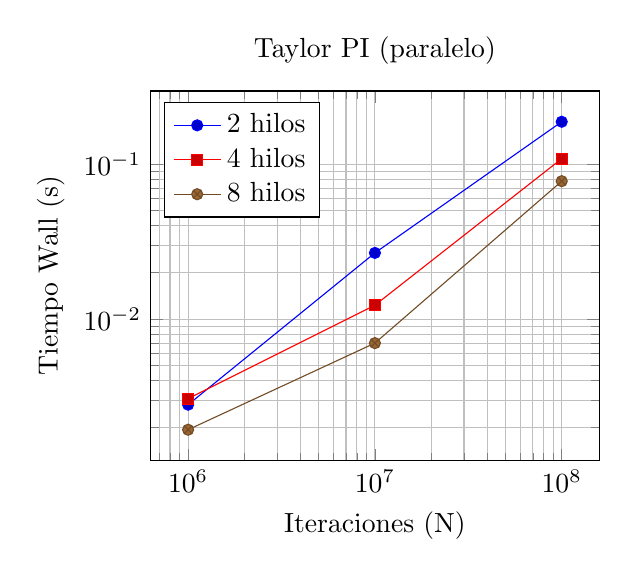
\begin{tikzpicture}
\begin{loglogaxis}[
    width=0.6\textwidth,
    xlabel={Iteraciones (N)},
    ylabel={Tiempo Wall (s)},
    title={Taylor PI (paralelo)},
    legend pos=north west,
    grid=both
]
\addplot coordinates {(1e6,0.0028035) (1e7,0.0267203) (1e8,0.187539885)};
\addlegendentry{2 hilos}
\addplot coordinates {(1e6,0.0030669) (1e7,0.0122906) (1e8,0.108343164)};
\addlegendentry{4 hilos}
\addplot coordinates {(1e6,0.0019328) (1e7,0.0069969) (1e8,0.077586926)};
\addlegendentry{8 hilos}
\end{loglogaxis}
\end{tikzpicture}
\caption{Tiempo de ejecución Wall para Taylor PI con distintos hilos}
\end{figure}

Observaciones:
\begin{itemize}
    \item El tiempo Wall disminuye significativamente al aumentar los hilos.
    \begin{itemize}
        \item Ejemplo en $10^8$: pasa de $0.187 s$ (2 hilos) $\rightarrow$ $0.077 s$ (8 hilos).
    \end{itemize}
    \item El tiempo CPU se mantiene relativamente constante (porque refleja el trabajo total hecho por todos los hilos).
    \item La precisión mejora con más iteraciones, y el error absoluto baja hasta el orden de $10^{-9}$
\end{itemize}

\textbf{Conclusión}: la paralelización escala muy bien en este algoritmo (casi ideal).

\newpage

\section*{Resultados \texttt{carlopi.cpp} (paralelo -- Monte Carlo)}

\begin{longtable}{>{\raggedright}p{2cm} >{\raggedright}p{1cm} 
>{\centering\arraybackslash}p{3cm} 
>{\centering\arraybackslash}p{3cm} 
>{\centering\arraybackslash}p{2cm} 
>{\centering\arraybackslash}p{3cm}}
\toprule
Iteraciones (N) & Hilos & Tiempo CPU (s) & Tiempo Wall (s) & Valor estimado $\pi$ & Error absoluto \\
\midrule
\endfirsthead
\toprule
Iteraciones (N) & Hilos & Tiempo CPU (s) & Tiempo Wall (s) & Valor estimado $\pi$ & Error absoluto \\
\midrule
\endhead
1e6 & 2 & 0.47819 & 0.241579655 & 3.142600 & 0.001007346 \\
1e6 & 4 & 0.64658 & 0.175579842 & 3.140444 & 0.001148653 \\
1e6 & 8 & 0.94419 & 0.126774304 & 3.140340 & 0.001252653 \\
1e7 & 2 & 4.61655 & 2.320695875 & 3.141303 & 0.000289453 \\
1e7 & 4 & 6.69396 & 1.698227549 & 3.141563 & 2.9053589e-05  \\
1e7 & 8 & 9.39104 & 1.233206821 & 3.141708 & 0.000115346 \\
1e8 & 2 & 50.4320 & 25.42126513 & 3.14185916 & 0.000266506 \\
1e8 & 4 & 69.4330 & 17.56811539 & 3.14148572 & 0.000106933 \\
1e8 & 8 & 92.9908 & 12.45675765 & 3.1411492 & 0.0004434535 \\

\bottomrule
\end{longtable}

\begin{center}
    \href{https://github.com/jucollas/parallel-programming/blob/main/submit-I/carlopi.cpp}{\faGithub\ \texttt{carlopi.cpp} in GitHub}
\end{center}

\begin{figure}[H]
\centering
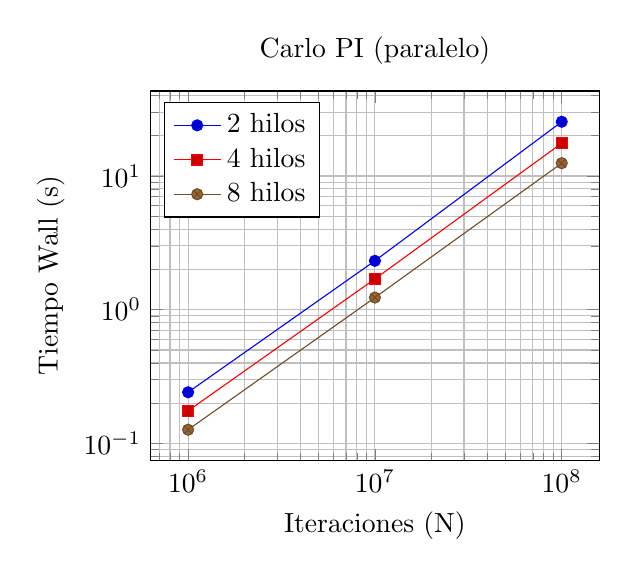
\begin{tikzpicture}
\begin{loglogaxis}[
    width=0.6\textwidth,
    xlabel={Iteraciones (N)},
    ylabel={Tiempo Wall (s)},
    title={Carlo PI (paralelo)},
    legend pos=north west,
    grid=both
]
\addplot coordinates {(1e6,0.241579655) (1e7,2.320695875) (1e8,25.42126513)};
\addlegendentry{2 hilos}
\addplot coordinates {(1e6,0.175579842) (1e7,1.698227549) (1e8,17.56811539)};
\addlegendentry{4 hilos}
\addplot coordinates {(1e6,0.126774304) (1e7,1.233206821) (1e8,12.45675765)};
\addlegendentry{8 hilos}
\end{loglogaxis}
\end{tikzpicture}
\caption{Tiempo de ejecución Wall para Carlo PI con distintos hilos}
\end{figure}

Observaciones:
\begin{itemize}
    \item  El tiempo Wall sí mejora con más hilos, pero no tanto como en Taylor.
    \begin{itemize}
        \item Ejemplo en $10^8$: $25.4 s$ (2 hilos) → $12.4 s$ (8 hilos) $\rightarrow$ $2x$ más rápido, pero no lineal. 
    \end{itemize}
    \item  El tiempo CPU crece notablemente con los hilos: muestra overhead de sincronización o gestión de threads.
    \item La precisión mejora con las iteraciones, pero sigue limitada por la naturaleza estocástica del método.
\end{itemize}
\textbf{Conclusión}: paraleliza, pero con eficiencia más baja que Taylor.

\newpage



\section*{Resultados \texttt{montepi.cpp} (secuencial -- Monte Carlo)}

\begin{longtable}{>{\raggedright}p{3cm} >{\raggedright}p{1cm} 
>{\centering\arraybackslash}p{3cm} 
>{\centering\arraybackslash}p{3cm} 
>{\centering\arraybackslash}p{3cm} 
>{\centering\arraybackslash}p{3cm}}
\toprule
Iteraciones (N) & Tiempo CPU (s) & Tiempo Wall (s) & Valor estimado $\pi$ & Error absoluto \\
\midrule
\endfirsthead
\toprule
Iteraciones (N) & Tiempo CPU (s) & Tiempo Wall (s) & Valor estimado $\pi$ & Error absoluto \\
\midrule
\endhead
1e6  & 0.35890 & 0.3608 & 3.14064 & 0.000952654 \\
1e7  & 3.79702 & 3.8192 & 3.14157 & 2.74536e-05 \\
1e8  & 38.3042 & 38.5914 & 3.1416 & 8.66641e-06 \\
\bottomrule
\end{longtable}

\begin{center}
    \href{https://github.com/jucollas/parallel-programming/blob/main/submit-I/montepi.cpp}{\faGithub\ \texttt{montepi.cpp} in GitHub}
\end{center}

\begin{figure}[H]
\centering
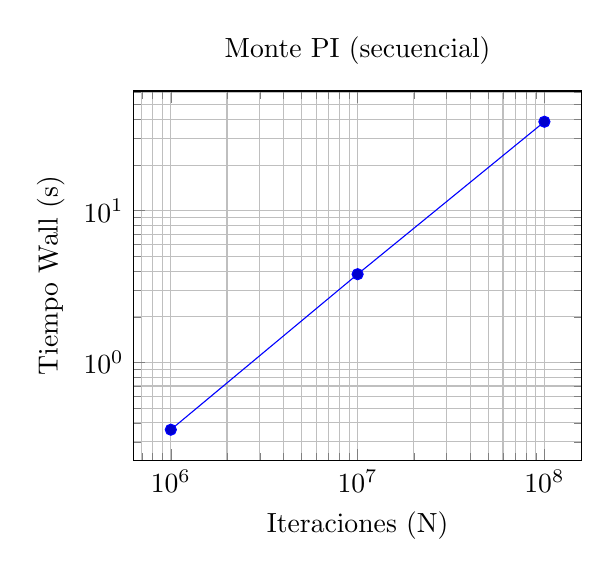
\begin{tikzpicture}
\begin{loglogaxis}[
    width=0.6\textwidth,
    xlabel={Iteraciones (N)},
    ylabel={Tiempo Wall (s)},
    title={Monte PI (secuencial)},
    grid=both
]
\addplot coordinates {(1e6,0.3608) (1e7,3.8192) (1e8,38.5914)};
\end{loglogaxis}
\end{tikzpicture}
\caption{Tiempo de ejecución Wall para Monte PI secuencial}
\end{figure}

Observaciones:
\begin{itemize}
    \item Escala de manera lineal con las iteraciones (tiempo se multiplica ~10x cuando las iteraciones suben 10x).
    \item Mucho más lento que Taylor para alcanzar la misma precisión.
    \begin{itemize}
        \item Ejemplo: en $10^8$, tarda $38 s$ (secuencial) vs $0.07–0.18$ s (Taylor paralelo).
    \end{itemize} 
\end{itemize}
\textbf{Conclusión}: el método secuencial Monte Carlo es poco competitivo en precisión/tiempo frente a los paralelos.

\newpage

\section*{Comparación General de los Métodos}

\subsection*{1. Precisión}

\textbf{Taylor (paralelo):} \\
El error absoluto decrece rápidamente con las iteraciones: llega al orden de $10^{-9}$ en $10^{8}$. 
Esto lo convierte en el método más preciso y estable. \\

\textbf{Carlo (paralelo, Monte Carlo):} \\
La precisión mejora con las iteraciones, pero de manera mucho más lenta. 
Incluso en $10^{8}$, el error se mantiene alrededor de $10^{-4}$ -- $10^{-5}$. 
Está limitado por la naturaleza aleatoria del método. \\

\textbf{Monte (secuencial, Monte Carlo):} \\
Similar al Carlo paralelo en precisión, pero más lento. 
A $10^{8}$, obtiene error cercano a $10^{-5}$. \\

\textbf{Conclusión en precisión:} Taylor domina, los métodos Monte Carlo son menos competitivos. 

\subsection*{2. Escalabilidad y tiempos de ejecución}

\textbf{Taylor paralelo:} \\
Escala casi ideal con el número de hilos. 
Ejemplo con $10^{8}$ iteraciones: de 0.187 s (2 hilos) $\rightarrow$ 0.077 s (8 hilos), 
lo que representa aproximadamente un \textit{speedup} real de $2.4\times$. 
El tiempo de CPU se mantiene casi constante, lo que indica una paralelización eficiente. \\

\textbf{Carlo paralelo:} \\
Escala peor que Taylor debido al overhead de sincronización y la generación de números aleatorios. 
Ejemplo con $10^{8}$: de 25.4 s (2 hilos) $\rightarrow$ 12.4 s (8 hilos), 
equivalente a un \textit{speedup} real de $\sim 2\times$. 
El tiempo de CPU crece considerablemente, lo que refleja menor eficiencia. \\

\textbf{Monte secuencial:} \\
Escala linealmente con las iteraciones, al no incluir paralelismo. 
En $10^{8}$ iteraciones, tarda 38.6 s, siendo mucho más lento que ambos métodos paralelos. \\

\textbf{Conclusión en tiempos:} Taylor paralelo es el más eficiente; 
Carlo paralelo se beneficia del paralelismo pero no escala tan bien; 
Monte secuencial es el menos competitivo.

\begin{figure}[H]
\centering
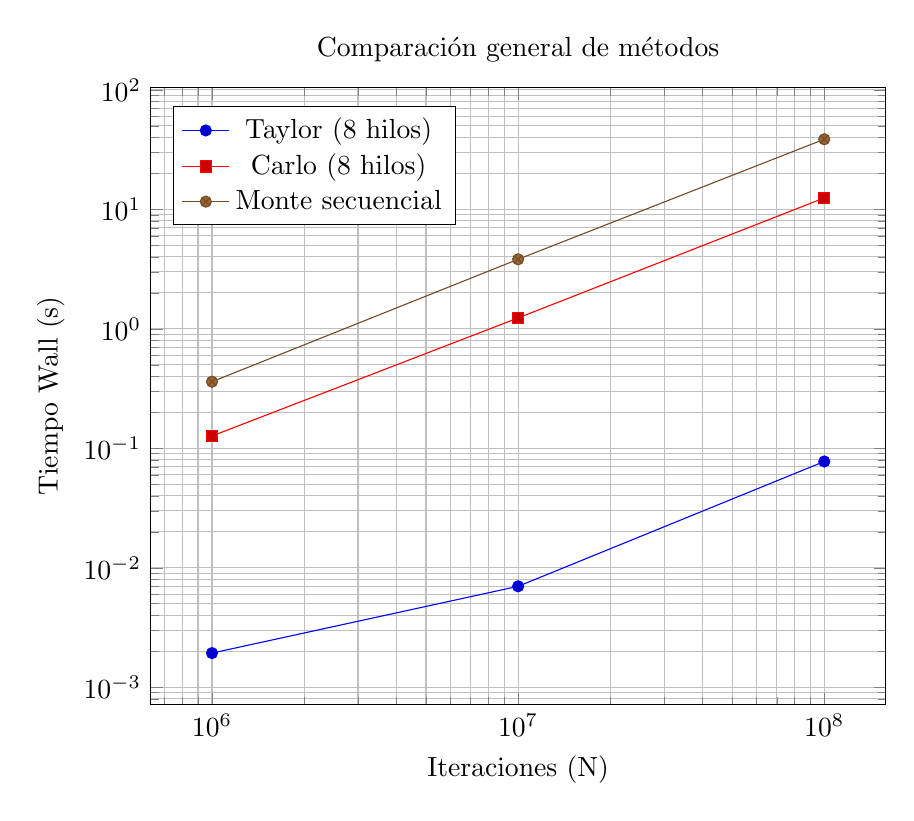
\begin{tikzpicture}
\begin{loglogaxis}[
    width=0.9\textwidth,
    xlabel={Iteraciones (N)},
    ylabel={Tiempo Wall (s)},
    title={Comparación general de métodos},
    legend pos=north west,
    grid=both
]

% Taylor (8 hilos)
\addplot coordinates {(1e6,0.0019328) (1e7,0.0069969) (1e8,0.077586926)};
\addlegendentry{Taylor (8 hilos)}

% Carlo (8 hilos)
\addplot coordinates {(1e6,0.126774304) (1e7,1.233206821) (1e8,12.45675765)};
\addlegendentry{Carlo (8 hilos)}

% Monte (Secuencial)
\addplot coordinates {(1e6,0.3608) (1e7,3.8192) (1e8,38.5914)};
\addlegendentry{Monte secuencial}
\end{loglogaxis}
\end{tikzpicture}
\caption{Comparación de tiempos Wall entre los tres métodos más representativos}
\end{figure}

\subsection*{Conclusión General}

\begin{itemize}
    \item \textbf{Taylor paralelo:} es el más rápido y preciso, además de escalar casi idealmente.
    \item \textbf{Carlo paralelo:} mejora con hilos, pero la eficiencia es más baja debido al \textit{overhead} y la aleatoriedad.
    \item \textbf{Monte secuencial:} funciona, pero es ineficiente comparado con los demás.
\end{itemize}

Para aplicaciones prácticas donde se busca \textbf{precisión y eficiencia}, Taylor paralelo es claramente superior. \\

Carlo paralelo solo tiene sentido en entornos donde el método estocástico sea requerido, como en \textbf{simulaciones probabilísticas}.


\end{document}
